
\graphicspath{ {mainmatter/Tanaka_2002/} }

\title*{2002: Multimodal Interaction in Music Using the Electromyogram and Relative Position Sensing}
\titlerunning{Multimodal Interaction in Music}

\author{Atau Tanaka and R. Benjamin Knapp}
\authorrunning{Tanaka and Knapp}

%\institute{Atau Tanaka \at Goldsmiths, University of London \\ original affiliation: Sony Computer Science Laboratories Paris\email{a.tanaka@gold.ac.uk}
%\and R. Benjamin Knapp \at Virginia Tech  \\ original affiliation: Moto Development Group  \email{benknapp@vt.edu}}
%
%
\maketitle

\abstract*{This paper describes a technique of multimodal, multichannel control of electronic musical devices using two control methodologies, the electromyogram (EMG) and relative position sensing. Requirements for the application of multimodal interaction theory in the musical domain are discussed. We introduce the concept of bidirectional complementarity to characterize the relationship between component sensing technologies. Each control can be used independently, but together they are mutually complementary. This reveals a fundamental difference from orthogonal systems. The creation of a concert piece based on this system is given as example.}

\section{Introduction}

Use of multiple axes of control in computer music performance is widespread. These systems typically use orthogonal bases to maximize the number of degrees of freedom of control mapping from input to synthesis parameter \cite{Freed:2000a}. Work in the field of Human Computer Interaction (HCI) focusing on multimodal interaction has concentrated on the notion of \textit{fusion} of inputs from different domains towards a given task. This paper discusses musical implications of multimodal interaction research and proposes a musical model of \textit{bidirectional complementarity} that reconciles the convergent model of fusion and the divergent model of orthogonal axes.

\section{Review of Multimodal Interaction}

Multimodal interaction can be separated into a human-centered view and a system-centered view. The former is rooted in perception and communications channels---exploring modes of human input/output \cite{Schomaker:1995}. The system-centered view focuses on computer input/output modes \cite{Raisamo:1999}. 

From a system-centered view, a single input device could be analyzed to derive multiple interpretations or multiple input devices can combine to help accomplish a single task. This notion of \textit{fusion} can exist in one of several forms: \textit{lexical fusion}, related to conceptual binding; \textit{syntactic fusion}, dealing with combinatorial sequencing; \textit{semantic fusion}, to do with meaning and function \cite{Nigay:1993}. These types of fusion are prone to \textit{temporal constraints}, which at the highest level distinguish parallel input from sequential input. 

According to Oviatt, ``the explicit goal [of multimodal interaction] is to integrate complementary modalities in a manner that yields a synergistic blend such that each mode can be capitalized upon and used to overcome weaknesses in the other mode'' \cite{Oviatt:2003} This is not the same as fusion. The interactions complement each other, not necessarily fuse with each other. 

Oviatt and other authors focus on restrictive, high stress, or mobile environments as settings which have a greater than normal need for multimodal interaction. The live musical performance environment clearly falls into this category.  This paper will focus on two modes of interaction that meet Oviatt's stated goal of complementary multimodal interaction in a mobile, high-pressure environment.



\section{The Electromyogram (EMG) / Position Sensing System}


The EMG is a biosignal that measures the underlying electrical activity of a muscle under tension (gross action potentials) using surface recording electrodes \cite{Criswell:2010}.  With a complexity approaching recorded speech, this electrical activity is rich in information about the underlying muscle activity.  Complex patterns found in the EMG can be used to detect underlying muscle gestures within a single recording channel \cite{Heinz:1996} quite similar to recognizing words spoken within continuous speech.  For example, individual finger motion can be recognized from a single channel of EMG recorder on the back of the forearm \cite{Putnam:1993}. While it is clear that this gesture recognition could be used to create a discrete event controller, it is unclear yet whether this will be a creatively useful for musical interaction.   

For several years, however, the overall dynamic energy of the EMG has been used as an expressive continuous controller \cite{Knapp:1990,Lusted:1996}. This is analogous to using the loudness of the voice as a controller. The analogy falls apart, however, when one understands the ``naturalness'' of the interaction of EMG.  Muscle tension conveys not just emotion, like the amplitude of the human voice, but the natural intentional actions of the muscle being recorded.  Using multiple sensors, the interaction of multiple EMGs can create a multichannel continuous controller that has no analogy.  The temporal interaction of these channels, which represent places of tension on the body, enables ``gestures'' of spatial tension patterns.

\begin{figure}[!htbp]
\centering
  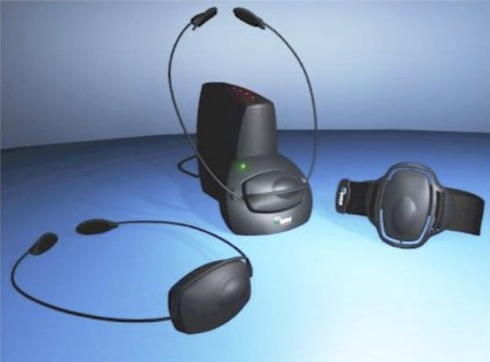
\includegraphics[width=\columnwidth]{figures/emginterface.jpg}
  \caption{EMG and Gyro-based Position Controller: Arm Bands, Head Bands, and Base.}
  \label{Tanaka:fig:emgcontroller}
\end{figure}

It is extremely important for the performer to understand that the EMG measures muscle activity that might or might not reflect muscle motion \cite{Tanaka:1993}.  For example, if an EMG electrode array were placed above the bicep and the performer were holding a heavy object steady in the bent arm position, there would be a great deal of EMG activity, with no corresponding movement.   Conversely, the arm could be relaxed causing a subsequently large movement of the arm which would not be recorded by the EMG. Thus, EMG measures isometric (no motion) activity extremely well, but isotonic (motion, but no change in tension) activity relatively poorly. 
 
Localized motion sensors such as accelerometers, gyroscopes, or levelers are far superior in measuring isotonic activity than the EMG. Thus, the addition of motion sensing to EMG sensing could create multimodal interaction to make a more expressive and complete interface.

As will be discussed in detail below, these two modes of interaction, position and EMG, can be thought of as demonstrating Oviatt's bi-directional complementarity.  That is, ``position'' could be thought of as the primary control with tension augmenting or modifying the positional information.  Vice versa, tension could be the primary control with position augmenting or modifying.  While this combination would be powerful in itself, the fact that both the tension and positional information can be multichannel creates a highly fluid, multidimensional, multimodal interaction environment.
  
In the proposed system, EMG electrodes are used in conjunction with gyroscopic sensors. The EMG surface recording electrodes are both conventional electrolyte-based electrodes and  more avant-garde active dry electrodes that use metal bars to make electrical contact with the skin. The EMG signal is acquired as a differential electrical signal. Instrumentation amplifiers on the electrodes themselves amplify and filter the signal before transmitting to the main interface unit.

The gyroscope sensors utilize a miniature electromechanical system. The device measures rotation and inertial displacement along two orthogonal axes.
The EMG and gyroscope information are then digitized. The amplitude envelope of the EMG is extracted via a straightforward RMS calculation. The Gyroscope data is accumulated over time to derive relative position information.


\section{Applying Multimodel Interaction Principles To Musical Control}


\subsection{Music as Use Case for Multimodal HCI}


Music performance is an activity that is well suited as a target for multimodal HCI concepts. Musical instruments for computer music performance are typically free-standing interface systems separate from the host computer system. They are thus well suited to explore the area in between the \textit{human-centered} and \textit{system-centered} views mentioned above. As music is by nature a time-based form, it is a medium particularly suited for investigations of temporal constraints. 

Music is a nonverbal form of articulation that requires both logical precision and intuitive expression. Sensor-based interactive devices have found application as instruments that facilitate real time gestural articulation of computer music. Most research in this domain \cite{:2000c} has focused on the musical mapping of gestural input. Given this focus on coherent mapping strategies, research has generally tended to isolate specific sensor technologies, relating them to a particular mapping algorithm to study their musical potential. 

Some sensor based musical instrument systems have been conceived \cite{Waisvisz:1985} that unite heterogeneous sensing techniques. We can think of these systems as prototypical multimodal interfaces for computer music. Such instruments might unite discrete sensors (such as switches) on the same device that also contains a continuous sensor (such as position). Operation of the continuous sensor could have different musical effect depending on the state of the discrete sensor, creating multiple modes for the use of a given sensor.


\subsection{Complementarity}


Seen in this light, traditional musical instruments can be thought of as multimodal HCI devices. Following the example given above, a piano has keys that discretize the continuous space of sound frequency. Pedals operated by the feet augment the function of the keys played by the fingers. Playing the same key always sounds the same note, but that articulates normally, muted, or sustained, depending on the state of the left and right pedals. This is a case of simple complementarity, where a main gesture is augmented by a secondary gesture.

With a stringed instrument such as the violin, multiple modes of interaction are exploited on single limb types. Bowing with one arm sets a string into vibration. Fingering with the hand on the other arm sets the base frequency of that same string. Meanwhile, multiple modes of interaction on the fingering hand enrich the pitch articulation on the string. Placing the finger on the string determines the basic pitch. Meanwhile, vibrato action with that same finger represents action with the same member in an orthogonal axis to modulate the frequency of the resulting sound. 

A case of co-dependent complementarity is seen in a woodwind instrument such as the clarinet. Two modes of interaction with the instrument work in essential combination to allow the performer to produce sound---a blowing action creates the air pressure waves while a fingering action determines the frequency. This is also a case where the two modes of interaction become more distinct one from the other: one is an interface for the mouth while the other is an interface for the hands. These two modes of interaction fuse to heighten our capability on the instrument. The complementarity is of a more equal nature than the pedal of a piano augmenting the articulation of the fingers. However, the complementarity remains unidirectional: the breath is still the main gesture essential for producing sound while the fingers augment the frequency dimension of articulation. Breathing without fingering will still produce a sound whereas fingering without breathing will not produce the normal tone associated with the clarinet.

With these examples, we observe that notions of multimodal interaction are present in traditional musical instrument technique. However, the nature of the complementarity tends to be unidirectional.

 
\subsection{Bidirectional Complementarity}

 
 There are two directions in which the notion of complementarity can be expanded. In the cases described above, discrete interventions typically augment a continuous action (albeit in the case of violin vibrato it is the converse).  One case in traditional musical performance practice that approaches use of two continuous modes is with conducting. The conductor articulates through arm gestures, but targets via gaze in a continuous visual space \cite{Usa:1998}.  However, the complementarity is still unidirectional---by gazing alone, the conductor is not accomplishing his task. The gaze direction supplements the essential conducting action.

The two sources of interaction in the system we propose, position sensing and EMG, are independent but not orthogonal, creating the possibility of \textit{bidirectional complementarity}. Each mode of interaction is sufficiently robust to be a freestanding mode of gesture--sound articulation. Musical instruments have been built using EMG alone and position sensing alone. Yet put in a complementary situation, each mode can benefit and expand on its basic range of articulation. EMG can complement position: Position/movement sensing can create the basic musical output while EMG can modulate this musical output to render it more expressive. Position can complement EMG: EMG can create the basic musical output while position sensing can create a Cartesian ``articulation space'' in which similar EMG trajectories can take on different meaning according to position.

  \begin{figure}[!htbp]
  \centering
  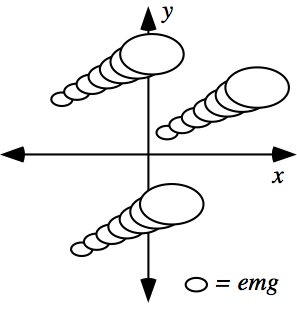
\includegraphics[scale=1]{figures/bidirectionalA.png}
  \caption{Bidirectional complementarity A: Position data complementing EMG gesture.}
  \label{Tanaka:fig:bidirectionalA}
\end{figure}

  \begin{figure}[!htbp]
  \centering
  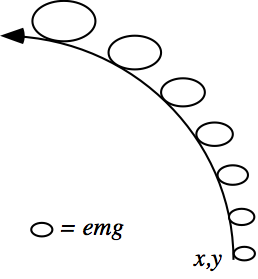
\includegraphics[scale=1]{figures/bidirectionalB.png}
  \caption{Bidirectional complementarity B: EMG data complementing positional displacement gesture.}
  \label{Tanaka:fig:bidirectionalB}
\end{figure}
 
\section{Requirements For Multimodal Musical Interaction}


\subsection{Efficiency of articulation and communication}


The net effect of expanding a sensor-based musical instrument system to be a multimodal interface must be a beneficial one. Judging the benefits of such enhanced interactivity in music differs from evaluating efficacy of task-oriented procedures. As music blends a subjective element to technical execution, evaluation of the system must also be considered on these multiple levels. 

\subsection{Multitasking vs. Multimodal}


Divergent multitasking should not be confused with focused multimodal interaction. For example, driving a car and talking on a mobile phone simultaneously is a case of the former. In such a situation, each activity is in fact hampered by the other---rather than heightening productivity, the subject finishes by executing both tasks poorly. Focused multimodal interaction should operate in a beneficial sense. If there are shortcomings in one mode, they should be compensated by enhancement \textit{afforded} by the other. As mentioned previously, this notion of \textit{mutual compensation} is a fundamental concept in multimodal HCI theory \cite{Oviatt:2003}. To what extent does it apply to musical practice?

Music as a performative form maintains criteria distinct from the pure efficiency standards of productivity studies. States of heightened musical productivity can be considered musically unsatisfying. In the case of a mechanical one-man-band, a fantastic mechanical apparatus is constructed to allow one person to play all the instruments of a band---from the various drums and cymbals to trumpet to organ. Caricatures of such a contraption evoke images of a musically silly situation. Why should a system optimized to allow a single user to interact with multiple musical instruments be considered a musical joke? Because there is the implicit understanding that the resulting music will be less effective than a real band of separate instruments. 

This example follows to some degree the example of driving and telephoning. By trying to do many things, one finishes but doing them all poorly. However, while driving and telephoning are distinct tasks, precluding its consideration as multimodal interaction, the one-man band can be considered a single musical device with multiple points of interaction. While the goal at hand is the single task of making music, this particular case of multiple modes is a musically unsuccessful one. 


\subsection{Defining a Successful Multimodal Interface}


A set of goals, then, needs to be put forth to help evaluate the effectiveness of musical interaction. The example above points out that maximizing the amount of pure productivity is not necessarily a musically positive result. Success of interactivity in music needs to be considered from the perspectives of both the performer and the listener. The goal is to attain musical satisfaction for each party. For the performer, this means a sense of articulative freedom and expressivity. The interfaces should provide modes of interaction that are intuitive to allow the performer to articulate his musical intention (control) at the same time allow him to ``let go.'' For the listener, computer based sounds are typically a family of sounds with little grounding in associative memory. Making sense of the gesture-sound interaction is a first requirement for achieving musical satisfaction \cite{Tanaka:2000}. However, at some moment, the audience also must be free to let go and have the possibility to forget the technical underpinnings of the action at hand and to appreciate the musical situation at a holistic level. A successful interactive music system should satisfy this level of intuition both for the performer and for the listener.

\subsection{Intuition}


This description of musical requirements outlined above point out likely criteria that need to be fulfilled at the interface level. Clarity of interaction is a fundamental requirement that is the basis of communication \cite{Tanaka:2000}---for feedback from the instrument back to the performer, and for transmission to the listener. However clarity alone is not enough---in fact an overly simplistic system will quickly be rendered banal. Interaction clarity can then perhaps be considered as an interim goal towards a more holistic musical satisfaction. The interfaces and modes of interactions then must be capable of creating a transparent situation where in the ideal situation the interface itself can be forgotten. By functioning at the level of intuition that allows performer and listener perception to overcome the mechanics of interaction, a musical communicative channel is established that is catalyzed by the modes of interaction, but not hindered by them.

\subsection{Expansion vs. Fusion}


While multimodal HCI discussion often focuses on \textit{fusion}, musical performance can exhibit different needs. A musical goal may not be so straightforward as the contribution of several interactions to a single result. Instead, articulative richness is a musical a goal that can be defined as different modes of interaction are contributing to distinct musical subtasks \cite{Tanaka:2001a}. The multiple modes of interaction allow simultaneous access to these articulation layers, enhancing the expressive potential of the performer. Seen in this light, multiple modes of interaction do not necessarily need to fuse towards one task, but can expand the potential of a musical gesture.  Thus complementarity is more important than fusion. 

\section{Application To Live Performance}


To demonstrate the capability of the multimodal, multichannel system proposed in this paper to enhance musical composition and performance, the authors have undertaken the development of a concert piece using EMG and relative position sensing. The piece, entitled \textit{Tibet}, includes an acoustical component in addition to the multimodal gesture sensing.  The acoustical component is created by circular bowing of resonant bowls. These bowls will be separated in space as well as pitch. These acoustic sounds, created by physical interaction, are extended by sampling and processing. This extended sonic vocabulary is articulated using a combination of gestures extracted from muscle and position sensors placed on the performer's arms. The results are complex textures in space, frequency, and time.  

  \begin{figure}[!htbp]
  \centering
  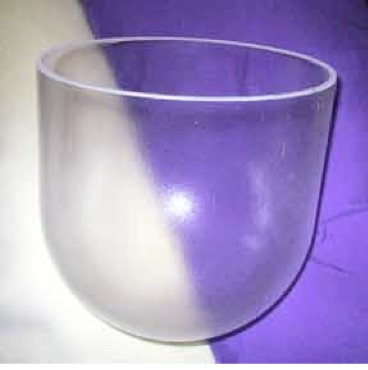
\includegraphics[scale=0.5]{figures/bowl.jpg}
  \caption{Acoustical crystal bowl .}
  \label{Tanaka:fig:crystalbowl}
\end{figure}

The piece explores the interstitial spaces between acoustic sound and electronic sound, between movement and tension, between contact and telepathy. Multiple, complimentary modes of interaction are called upon to explore these spaces. Physical contact elicits acoustical sound. These gestures are tracked as EMG data, allowing an electronic sonic sculpting that augments the original acoustic sound. In a second mode, the biosignal can continue to articulate sounds in the absence of physical contact with the bowls. In a third mode, the EMG based articulation of the sound is itself then augmented by position sensors. The position sensors give topological sense to the otherwise tension-based EMG data. Similar muscle gestures then take on different meaning in different points in space. Here we explore the articulatory space of complementary sensor systems. The piece finishes with the return of physical contact, keeping the EMG and position sensing in a unified gestural expression.


\section{Conclusions}


The approach introduced in this paper combines criteria established in the two fields of multimodal HCI research and gestural music interface research. With this we have defined design goals for what constitutes a musically successful implementation of multimodal interaction. We believe that the system proposed in this paper, using EMG in conjunction with relative position sensing, achieves the outlined goals of a successful multimodal musical interface:

\begin{enumerate}
\item Each of the component modes are intuitive interfaces 
\item The multimode context leverages the richness of each interface to expand the articulative range of the other
\item The two interfaces are independent and yet exhibit bi-directional complementarity

\end{enumerate}

We have reviewed the fundamentals of multimodal human computer interaction as applied to musical performance. In this paper, we have described specificities of music that make it apt for the application of multimodal HCI concepts. We have indicated other characteristics of music that allow us to expand on the single task orientation of classical multimodal HCI research. We proposed a multimodal gestural music system based on biosignals and relative position sensing. We introduce the notion of \textit{bidirectional complementarity} that defines the interdependent relationship between the two sensing systems and establishes the richness of interaction required and afforded by music.  Finally, we have described a musical piece that demonstrates the interaction capabilities of the proposed system.
 

\begin{acknowledgement}
\
The authors would like to thank Sony CSL and Moto Development Group for supporting this work.
\end{acknowledgement}

\section*{Author commentary: Multimodal musical interaction, a decade later}
\paragraph{Atau Tanaka and R. Benjamin Knapp}

The technologies we enthusiastically wrote about in 2002 are now readily available, and are quickly becoming mainstream. There are consumer EMG devices that have been Kickstarted\footnote{\url{http://www.myo.com}} as well as devices that expand the use of electrophysiology from the somatic (EMG) to the autonomic nervous system (signals such as the EDA and HR).\footnote{\url{http://www.empatica.com}} These consumer-grade devices can give clean enough data to be useful in research, opening up the range of potential creative applications in NIME. Many of these devices integrate physical sensing alongside physiological sensing, making them multimodal. The ideas we wrote about over a decade ago, on the use of multiple modes of interaction for music, have arrived in commercially available technologies, and are available to all musicians and artists. This increased accessibility has not lessened the research challenges, however, and the core scientific imperatives remain. How can we best make use of multiple modes of interaction with gestural input to create rich musical results? As we deepen our study of multimodal interaction and connect that to human capabilities of intermodal perception, we sharpen our research focus. 

%Meanwhile, the more we know, the more there is to verify, risking to turn the research incremental.

The distinction we made in the original paper between ``human-centered'' and ``system-centered'' views are not as clear cut today as they used to be. In fact they are fundamentally intertwined in the design of modern interactive systems. Research in infant cognitive development shows that intermodal perception is innate, as well as learned. 
% \cite{thelen1996dynamic}. 
This means that we naturally use multiple sensory modes to make sense of events in the world. At the same time, we learn new links, and are capable of forming cross-modal mappings that are not inherent. Increasingly, interaction design is informed by this knowledge of cognitive processes. Today, we build interactive systems that support these human capabilities, making the system-view inherently human-centric.

The focus on ``control'' in the original paper belies the era in which it was written. The turn of the  new millennium, coming out of two decades of MIDI, was a technologically more deterministic time. Today we are less positivist, preferring to look at human-machine relationships where control may not be desired nor possible. Indeed, the evolution of this work to include affect measurement has challenged what the word, control, means in the context of the modern digital musical instrument. Input/output mappings go beyond the classical one-to-many and many-to-one paradigms to also include direct sonification, audification, input modeling, and feature mapping.

Despite these advancements in thinking, the core literature on multimodal interaction reviewed in the paper continues to be essential reading. They remind us of important concepts such as fusion, temporal constraints, and complementarity. In our present-day, lightspeed scans of Google Scholar and the ACM Digital Library, it's easy to overlook this foundational literature. Re-reading our own paper even as we continue these lines of research was an eye opener for us.  There have since been important advancements in novel methods, such as the use of sensory substitution in the interface \cite{Bach-y-Rita:2003}, and the codification of multimodal interaction in methodological frameworks \cite{Norris:2004}.

The sections relating multimodal concepts to  musical practice are, in retrospect and in the spirit of self-criticism, quaintly naive. The comparisons we made at the time to piano and violin performance practice and conducting are in fact examples of multi-channel input and not multimodal interaction \textit{per se}. Indeed, the section distinguishing musical practice from task based performance, though true, is speculative, and shows the romantic possibility of research back then. Today, the availability of ready tools, and the advancement of research in these topics fence us into forms of rigor, that, if not intellectually constraining, make us more incremental in the claims we put forth.

The core work reported in the original paper is, we believe, still useful today. Physiological sensing via the EMG can complement inertial position sensing, and vice versa. Bi-directional complementarity is a good way to frame the mutually reinforcing nature of these multimodal relationships.

We have since continued this research. The EMG has been put in bi-modal contexts alongside biophysical sensing of the mechano-myogram (MMG) and we have studied the EMG in multimodal contexts with motion capture systems in addition to accelerometers. We have looked more closely at the EMG signal itself, in conjunction with the MMG \cite{Donnarumma:2013}, and to see how feature extraction can pre-process the bio-signal for subsequent machine learning analysis \cite{Caramiaux:2015}.  We have explored how EMG can be one component of an affective interface \cite{Knapp:2011}. We have studied how musicians and non-musicians can produce and reproduce gesture, reliably articulate expressive variation of gesture, and look at hardware and software's ability (and limits) in tracking this. Based on this, we build musical systems that are tuned to users' abilities, be they virtuostic, disabled, or lay performers.


\section*{Expert commentary: Human bodies, algorithms and intuition}
\paragraph{Marco Donnarumma}

In 2002, when this paper by Atau Tanaka and Ben Knapp was published, the NIME conference was just at its second edition. While the NIME community had been formalised only the year before, the uniquely inventive and cross-disciplinary spirit grounding the design and performance with new musical instruments had been nurtured since much longer \cite{Krefeld:1990,Moore:1988}. The individual and joint research by Tanaka and Knapp in particular has been seminal to different areas of NIME research: from gestural interaction to hardware design, from biomusic to mobile music. Tanaka and Knapp's approach to new musical instrument performance has been, and still is, as much idiosyncratic as innovative. They had been collaborating since the late 1980s, when Knapp and Hugh Lusted commissioned Tanaka the creation of the first musical piece for their bioelectrical musical interface, the Biomuse. In \textit{Kagami}, the related piece created by Tanaka and premiered in 1992 at CCRMA Stanford, Tanaka, Knapp and Lusted used armbands embedded with wet electrodes to capture electrical discharges from the performer's forearm and upper arm muscles, measured as electromyogram or EMG. The electrical signals were then digitized and translated into MIDI parameters modulating a Yamaha TG77 and a Korg Wavestation.

The design and performative approach of Tanaka, Lusted and Knapp expanded the breadth of gestural performance with NIME by enabling a kind of interaction between performer and instrument that Tanaka has termed \lq visceral\rq \cite{Tanaka:2011}. For Tanaka, visceral refers to the fact that the instrument's physiological sensing affords the capture of information on the performer's intention of movement, rather than how movement is performed in space. Tanaka and Knapp's approach evolved through the years and by 2002 they presented the paper in question, which proposes a framework for multimodal interaction in music performance using two sensing modalities, EMG and relative position sensing. Combining multimodal interaction methods, developed in the field of human-computer interaction (HCI), and gestural control of computer-based musical instrument,  the article discusses the use of those two independent, and yet complementary, sensing modalities to increase the level of expressive musical articulation available to the performer. The paper also offers insights on a practical application of the multimodal framework to \textit{Tibet}, a piece that was performed at the same conference. The article provided two major contributions to the NIME community. First, it formally introduced the basic properties of EMG sensing in the context of real-time musical interaction with computer-based instruments, a sensing modality that had been described on other occasions by the same authors, but not yet in the specific context of NIME. Second, it elaborated on a set of multimodal sensing methods in HCI and thus identified the most suitable for musical performance, that of bidirectional complementarity, where independent sensing modalities can take advantage from, and extend, each other. A light weakness of the paper lies in that the two ending sections bring the discussion to a hasty close, and we are left with an exciting prospect and only few hints of its potential in a real-world performance. The interested reader can refer to an online video excerpt of the related performance, \textit{Tibet},\footnote{\url{https://www.youtube.com/watch?v=O_z0hdS4umY}} by Atau Tanaka.

However, what makes this paper highly significant to our present community is, to my view, the way in which the contributions are framed. The article does not focus on technical insights on the use of biosignals or gyroscope data; rather, it contends the capacity of the proposed multimodal approach to create room for intuition, bodily skill, control and lack thereof, in musical gestural interaction. This is an approach to NIME performance that balances technical insight with bodily performance, algorithms with intuition. In the past years this kind of approach has increasingly lost currency in favour of primarily technical research into the affordances of new instruments. What we can abstract thus from Tanaka and Knapp's contribution is the importance of integrating technical findings and insights on bodily performance into our research methods. This can be done by considering the importance of corporeality to performance with computer-based musical instruments. Corporeality, meaning the physical, physiological and cultural basis of embodied practices, is a foundation of musical performance, and should therefore not be seen as a minor issue in our research and practise. Rather, technical research itself can be informed by looking at how technological instruments, algorithms and sound manipulations, not only bring forth new kinds of music, but also extend, hinder or alter the properties of the performer's and the listeners' bodies \cite{Hayles:1999,Henriques:2011}. 

